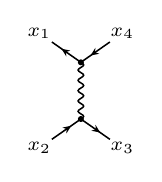
\begin{tikzpicture}[x=0.600cm, y=0.600cm, line width=0.550pt, baseline={([yshift=-0.6ex]0,0)}]
  \draw plot[smooth, tension=0.7] coordinates {(0.000,0.600) (0.042,0.573) (0.059,0.545) (0.042,0.518) (0.000,0.491) (-0.042,0.464) (-0.059,0.436) (-0.042,0.409) (0.000,0.382) (0.042,0.355) (0.059,0.327) (0.042,0.300) (0.000,0.273) (-0.042,0.245) (-0.059,0.218) (-0.042,0.191) (0.000,0.164) (0.042,0.136) (0.059,0.109) (0.042,0.082) (0.000,0.055) (-0.042,0.027) (-0.059,0.000) (-0.042,-0.027) (0.000,-0.055) (0.042,-0.082) (0.059,-0.109) (0.042,-0.136) (0.000,-0.164) (-0.042,-0.191) (-0.059,-0.218) (-0.042,-0.245) (0.000,-0.273) (0.042,-0.300) (0.059,-0.327) (0.042,-0.355) (0.000,-0.382) (-0.042,-0.409) (-0.059,-0.436) (-0.042,-0.464) (0.000,-0.491) (0.042,-0.518) (0.059,-0.545) (0.042,-0.573) (0.000,-0.600)};
  \draw (0.000,0.600) -- (-0.614,1.030);
  \fill (-0.410,0.887) -- (-0.309,0.724) -- (-0.312,0.819) -- (-0.222,0.848) -- cycle;
  \draw (0.000,-0.600) -- (-0.614,-1.030);
  \fill (-0.204,-0.743) -- (-0.392,-0.782) -- (-0.302,-0.811) -- (-0.306,-0.906) -- cycle;
  \draw (0.000,-0.600) -- (0.614,-1.030);
  \fill (0.410,-0.887) -- (0.309,-0.724) -- (0.312,-0.819) -- (0.222,-0.848) -- cycle;
  \draw (0.000,0.600) -- (0.614,1.030);
  \fill (0.204,0.743) -- (0.392,0.782) -- (0.302,0.811) -- (0.306,0.906) -- cycle;
  \fill (0.000,0.600) circle (0.064);
  \fill (0.000,-0.600) circle (0.064);
  \node[font=\scriptsize, inner sep=0pt, anchor=325] at (-0.688,1.082) {$x_{1}$};
  \node[font=\scriptsize, inner sep=0pt, anchor=35] at (-0.688,-1.082) {$x_{2}$};
  \node[font=\scriptsize, inner sep=0pt, anchor=145] at (0.688,-1.082) {$x_{3}$};
  \node[font=\scriptsize, inner sep=0pt, anchor=215] at (0.688,1.082) {$x_{4}$};
\end{tikzpicture}
\allowbreak\;{-}\; 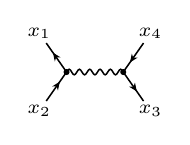
\begin{tikzpicture}[x=0.600cm, y=0.600cm, line width=0.550pt, baseline={([yshift=-0.6ex]0,0)}]
  \draw plot[smooth, tension=0.7] coordinates {(-0.600,0.000) (-0.573,0.042) (-0.545,0.059) (-0.518,0.042) (-0.491,0.000) (-0.464,-0.042) (-0.436,-0.059) (-0.409,-0.042) (-0.382,0.000) (-0.355,0.042) (-0.327,0.059) (-0.300,0.042) (-0.273,0.000) (-0.245,-0.042) (-0.218,-0.059) (-0.191,-0.042) (-0.164,0.000) (-0.136,0.042) (-0.109,0.059) (-0.082,0.042) (-0.055,0.000) (-0.027,-0.042) (0.000,-0.059) (0.027,-0.042) (0.055,0.000) (0.082,0.042) (0.109,0.059) (0.136,0.042) (0.164,0.000) (0.191,-0.042) (0.218,-0.059) (0.245,-0.042) (0.273,0.000) (0.300,0.042) (0.327,0.059) (0.355,0.042) (0.382,0.000) (0.409,-0.042) (0.436,-0.059) (0.464,-0.042) (0.491,0.000) (0.518,0.042) (0.545,0.059) (0.573,0.042) (0.600,0.000)};
  \draw (-0.600,0.000) -- (-1.030,0.614);
  \fill (-0.887,0.410) -- (-0.848,0.222) -- (-0.819,0.312) -- (-0.724,0.309) -- cycle;
  \draw (-0.600,0.000) -- (-1.030,-0.614);
  \fill (-0.743,-0.204) -- (-0.906,-0.306) -- (-0.811,-0.302) -- (-0.782,-0.392) -- cycle;
  \draw (0.600,0.000) -- (1.030,-0.614);
  \fill (0.887,-0.410) -- (0.848,-0.222) -- (0.819,-0.312) -- (0.724,-0.309) -- cycle;
  \draw (0.600,0.000) -- (1.030,0.614);
  \fill (0.743,0.204) -- (0.906,0.306) -- (0.811,0.302) -- (0.782,0.392) -- cycle;
  \fill (-0.600,0.000) circle (0.064);
  \fill (0.600,0.000) circle (0.064);
  \node[font=\scriptsize, inner sep=0pt, anchor=305] at (-1.082,0.688) {$x_{1}$};
  \node[font=\scriptsize, inner sep=0pt, anchor=55] at (-1.082,-0.688) {$x_{2}$};
  \node[font=\scriptsize, inner sep=0pt, anchor=125] at (1.082,-0.688) {$x_{3}$};
  \node[font=\scriptsize, inner sep=0pt, anchor=235] at (1.082,0.688) {$x_{4}$};
\end{tikzpicture}